\documentclass{standalone}
\usepackage{tikz}
\usetikzlibrary{patterns}
\usetikzlibrary{positioning}
\usetikzlibrary{patterns, positioning}
\usetikzlibrary{shapes.misc}
\usepackage[outline]{contour}
\contourlength{1.5pt} 
\usepackage[sfdefault]{ClearSans}

\begin{document}
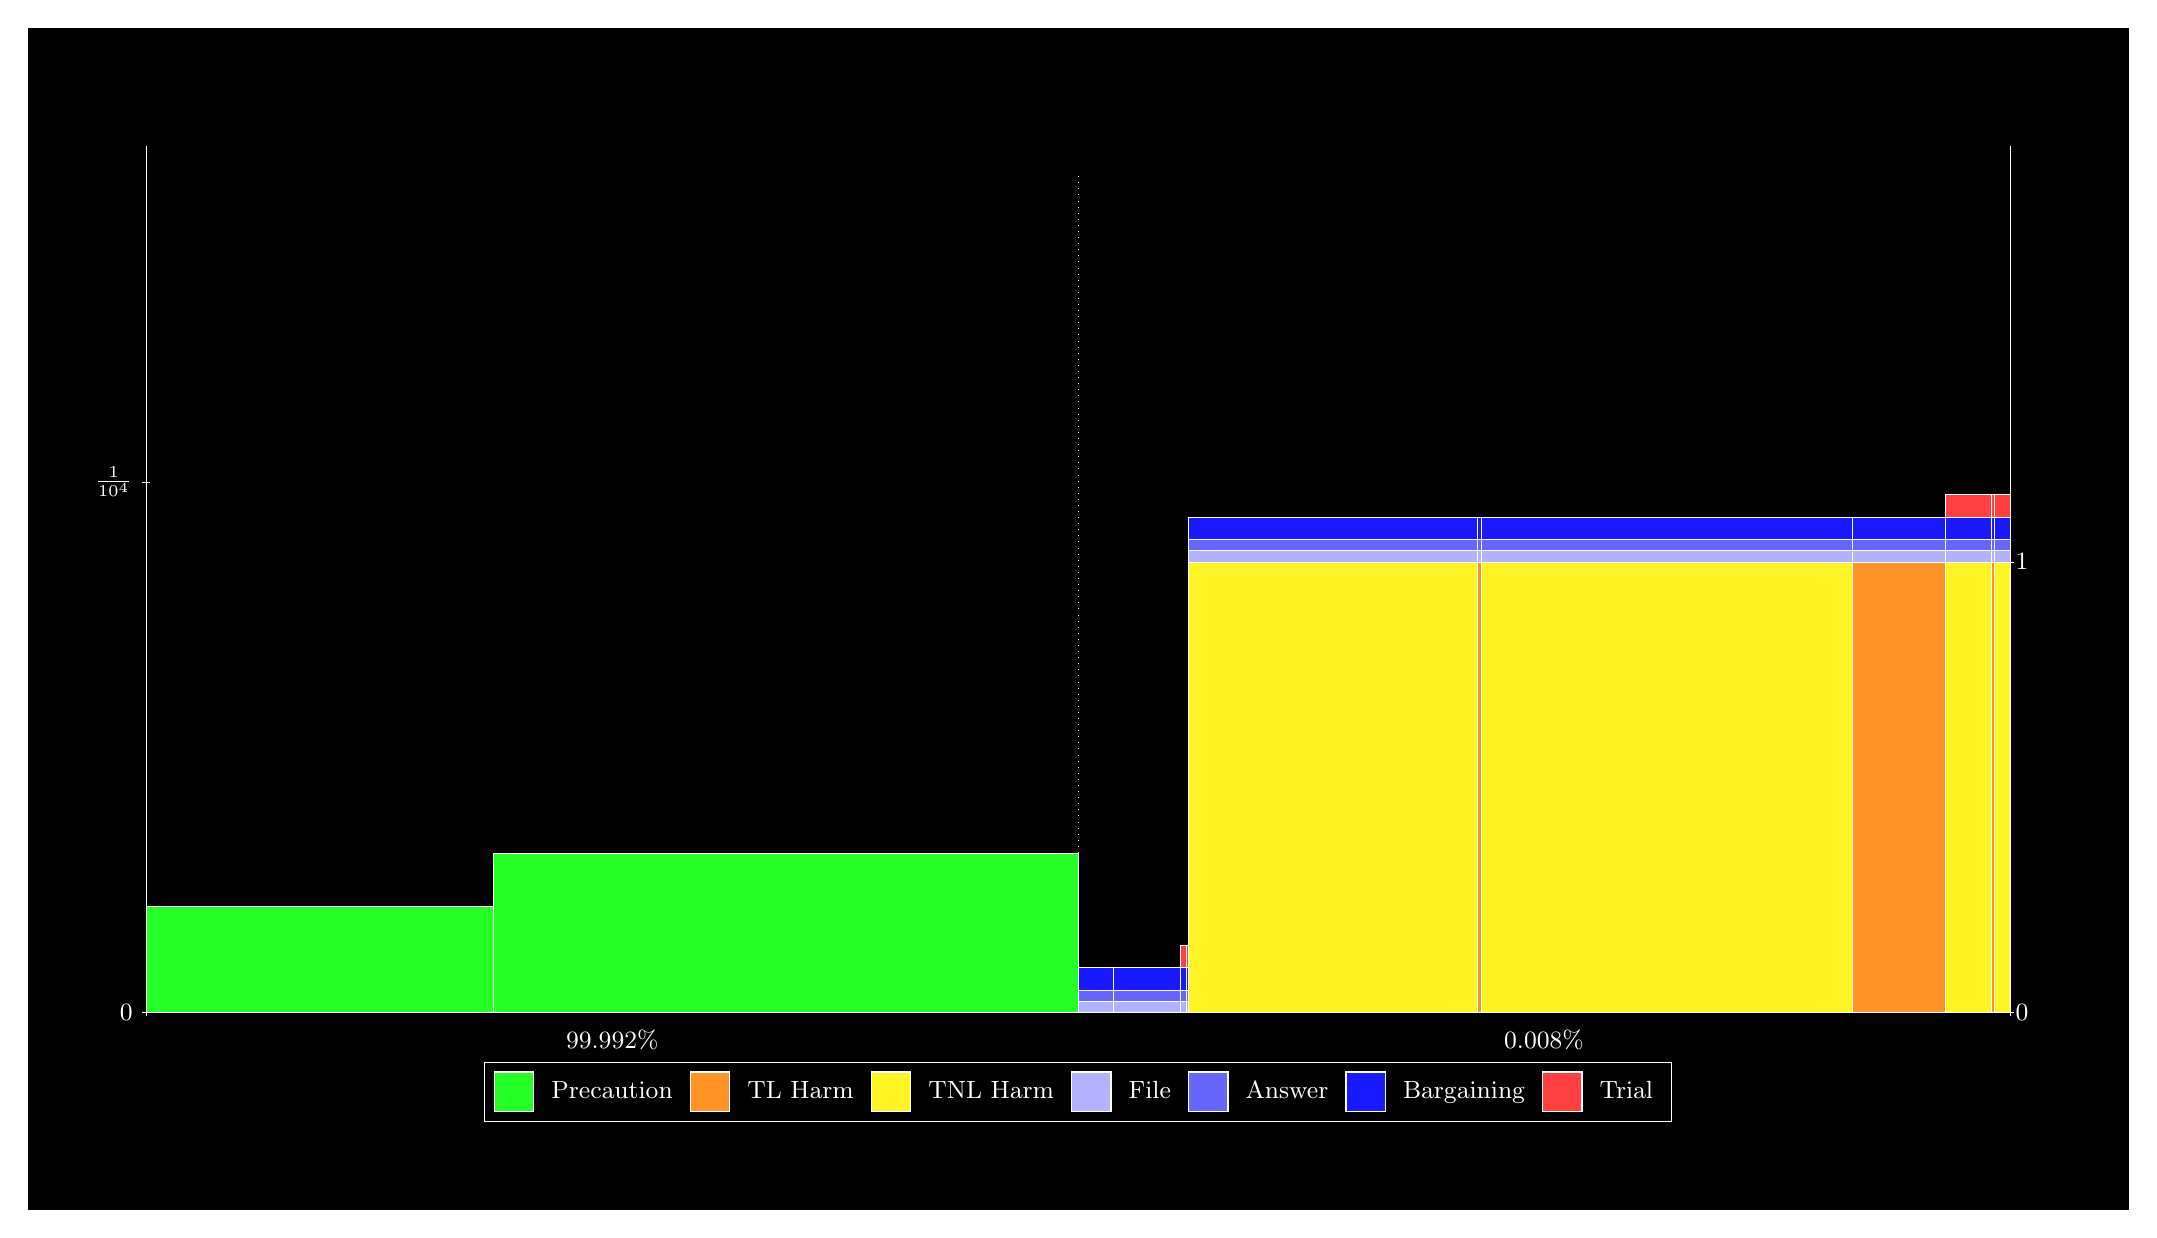
\begin{tikzpicture}
\draw[fill=black] (0,0) rectangle (26.667,15);
\draw[fill=green!85,draw=white,very thin] (1.5,2.5) rectangle (5.9116,3.8478);
\draw[fill=green!85,draw=white,very thin] (5.9116,2.5) rectangle (13.333,4.5217);
\draw[fill=green!85,draw=white,very thin] (13.333,2.5) rectangle (13.778,2.5001);
\draw[fill=blue!30,draw=white,very thin] (13.333,2.5001) rectangle (13.778,2.6432);
\draw[fill=blue!60,draw=white,very thin] (13.333,2.6432) rectangle (13.778,2.7862);
\draw[fill=blue!90,draw=white,very thin] (13.333,2.7862) rectangle (13.778,3.0724);
\draw[fill=green!85,draw=white,very thin] (13.778,2.5) rectangle (14.627,2.5002);
\draw[fill=blue!30,draw=white,very thin] (13.778,2.5002) rectangle (14.627,2.6432);
\draw[fill=blue!60,draw=white,very thin] (13.778,2.6432) rectangle (14.627,2.7863);
\draw[fill=blue!90,draw=white,very thin] (13.778,2.7863) rectangle (14.627,3.0724);
\draw[fill=green!85,draw=white,very thin] (14.627,2.5) rectangle (14.701,2.5001);
\draw[fill=blue!30,draw=white,very thin] (14.627,2.5001) rectangle (14.701,2.6432);
\draw[fill=blue!60,draw=white,very thin] (14.627,2.6432) rectangle (14.701,2.7862);
\draw[fill=blue!90,draw=white,very thin] (14.627,2.7862) rectangle (14.701,3.0724);
\draw[fill=red!75,draw=white,very thin] (14.627,3.0724) rectangle (14.701,3.3585);
\draw[fill=green!85,draw=white,very thin] (14.701,2.5) rectangle (14.728,2.5002);
\draw[fill=blue!30,draw=white,very thin] (14.701,2.5002) rectangle (14.728,2.6432);
\draw[fill=blue!60,draw=white,very thin] (14.701,2.6432) rectangle (14.728,2.7863);
\draw[fill=blue!90,draw=white,very thin] (14.701,2.7863) rectangle (14.728,3.0724);
\draw[fill=red!75,draw=white,very thin] (14.701,3.0724) rectangle (14.728,3.3586);
\draw[fill=green!85,draw=white,very thin] (14.728,2.5) rectangle (18.403,2.5001);
\draw[fill=yellow!85,draw=white,very thin] (14.728,2.5001) rectangle (18.403,8.2226);
\draw[fill=blue!30,draw=white,very thin] (14.728,8.2226) rectangle (18.403,8.3657);
\draw[fill=blue!60,draw=white,very thin] (14.728,8.3657) rectangle (18.403,8.5088);
\draw[fill=blue!90,draw=white,very thin] (14.728,8.5088) rectangle (18.403,8.7949);
\draw[fill=green!85,draw=white,very thin] (18.403,2.5) rectangle (18.455,2.5001);
\draw[fill=orange!85,draw=white,very thin] (18.403,2.5001) rectangle (18.455,8.2226);
\draw[fill=blue!30,draw=white,very thin] (18.403,8.2226) rectangle (18.455,8.3657);
\draw[fill=blue!60,draw=white,very thin] (18.403,8.3657) rectangle (18.455,8.5088);
\draw[fill=blue!90,draw=white,very thin] (18.403,8.5088) rectangle (18.455,8.7949);
\draw[fill=green!85,draw=white,very thin] (18.455,2.5) rectangle (23.165,2.5002);
\draw[fill=yellow!85,draw=white,very thin] (18.455,2.5002) rectangle (23.165,8.2227);
\draw[fill=blue!30,draw=white,very thin] (18.455,8.2227) rectangle (23.165,8.3658);
\draw[fill=blue!60,draw=white,very thin] (18.455,8.3658) rectangle (23.165,8.5088);
\draw[fill=blue!90,draw=white,very thin] (18.455,8.5088) rectangle (23.165,8.795);
\draw[fill=green!85,draw=white,very thin] (23.165,2.5) rectangle (24.344,2.5002);
\draw[fill=orange!85,draw=white,very thin] (23.165,2.5002) rectangle (24.344,8.2227);
\draw[fill=blue!30,draw=white,very thin] (23.165,8.2227) rectangle (24.344,8.3658);
\draw[fill=blue!60,draw=white,very thin] (23.165,8.3658) rectangle (24.344,8.5088);
\draw[fill=blue!90,draw=white,very thin] (23.165,8.5088) rectangle (24.344,8.795);
\draw[fill=green!85,draw=white,very thin] (24.344,2.5) rectangle (24.931,2.5001);
\draw[fill=yellow!85,draw=white,very thin] (24.344,2.5001) rectangle (24.931,8.2226);
\draw[fill=blue!30,draw=white,very thin] (24.344,8.2226) rectangle (24.931,8.3657);
\draw[fill=blue!60,draw=white,very thin] (24.344,8.3657) rectangle (24.931,8.5088);
\draw[fill=blue!90,draw=white,very thin] (24.344,8.5088) rectangle (24.931,8.7949);
\draw[fill=red!75,draw=white,very thin] (24.344,8.7949) rectangle (24.931,9.081);
\draw[fill=green!85,draw=white,very thin] (24.931,2.5) rectangle (24.965,2.5001);
\draw[fill=orange!85,draw=white,very thin] (24.931,2.5001) rectangle (24.965,8.2226);
\draw[fill=blue!30,draw=white,very thin] (24.931,8.2226) rectangle (24.965,8.3657);
\draw[fill=blue!60,draw=white,very thin] (24.931,8.3657) rectangle (24.965,8.5088);
\draw[fill=blue!90,draw=white,very thin] (24.931,8.5088) rectangle (24.965,8.7949);
\draw[fill=red!75,draw=white,very thin] (24.931,8.7949) rectangle (24.965,9.081);
\draw[fill=green!85,draw=white,very thin] (24.965,2.5) rectangle (25.167,2.5002);
\draw[fill=yellow!85,draw=white,very thin] (24.965,2.5002) rectangle (25.167,8.2227);
\draw[fill=blue!30,draw=white,very thin] (24.965,8.2227) rectangle (25.167,8.3658);
\draw[fill=blue!60,draw=white,very thin] (24.965,8.3658) rectangle (25.167,8.5088);
\draw[fill=blue!90,draw=white,very thin] (24.965,8.5088) rectangle (25.167,8.795);
\draw[fill=red!75,draw=white,very thin] (24.965,8.795) rectangle (25.167,9.0811);
\draw[white,very thin] (1.5,2.5) -- (1.5,13.5);
\draw[white,very thin] (1.45,2.5) -- (1.55,2.5);
\node[font=\small,text=white, anchor=east] at (1.45, 2.5) {0};
\draw[white,very thin] (1.45,9.2389) -- (1.55,9.2389);
\node[font=\small,text=white, anchor=east] at (1.45, 9.2389) {$\frac{1}{10^{4}}$};

\draw[white,dotted,very thin] (13.333,2.83) -- (13.333,13.17);
\draw[white,very thin] (25.167,2.5) -- (25.167,13.5);
\draw[white,very thin] (25.117,2.5) -- (25.217,2.5);
\node[font=\small,text=white, anchor=west] at (25.117, 2.5) {0};
\draw[white,very thin] (25.117,8.2225) -- (25.217,8.2225);
\node[font=\small,text=white, anchor=west] at (25.117, 8.2225) {1};

\draw[white,very thin] (1.5,2.5) -- (25.167,2.5);
\draw[white,very thin] (1.5,2.45) -- (1.5,2.55);
\node[font=\small,text=white, anchor=north] at (1.5, 2.45) {};
\draw[white,very thin] (25.167,2.45) -- (25.167,2.55);
\node[font=\small,text=white, anchor=north] at (25.167, 2.45) {};

\node[font=\small,text=white,anchor=south] at (7.4167, 1.9) {99.992\%};
\node[font=\small,text=white,anchor=south] at (19.25, 1.9) {0.008\%};
\draw (13.3333,2.5) node (B) {};
\begin{scope}[align=center]
\matrix[scale=0.5,draw=white,below=0.5cm of B,nodes={draw},column sep=0.1cm]{
\node[rectangle,draw,minimum width=0.5cm,minimum height=0.5cm,fill=green!85]{}; & \node[draw=none,font=\small,text=white]{Precaution}; &
\node[rectangle,draw,minimum width=0.5cm,minimum height=0.5cm,fill=orange!85]{}; & \node[draw=none,font=\small,text=white]{TL Harm}; &
\node[rectangle,draw,minimum width=0.5cm,minimum height=0.5cm,fill=yellow!85]{}; & \node[draw=none,font=\small,text=white]{TNL Harm}; &
\node[rectangle,draw,minimum width=0.5cm,minimum height=0.5cm,fill=blue!30]{}; & \node[draw=none,font=\small,text=white]{File}; &
\node[rectangle,draw,minimum width=0.5cm,minimum height=0.5cm,fill=blue!60]{}; & \node[draw=none,font=\small,text=white]{Answer}; &
\node[rectangle,draw,minimum width=0.5cm,minimum height=0.5cm,fill=blue!90]{}; & \node[draw=none,font=\small,text=white]{Bargaining}; &
\node[rectangle,draw,minimum width=0.5cm,minimum height=0.5cm,fill=red!75]{}; & \node[draw=none,font=\small,text=white]{Trial}; \\\\
};\end{scope}

\end{tikzpicture}
\end{document}